\documentclass[a4paper, 10pt, twoside]{article}
\usepackage[left=2cm, right=2cm, top=2cm, bottom=3cm]{geometry}
\usepackage{amsmath}
\usepackage[shortlabels]{enumitem}
\usepackage{bbold}
\usepackage{cases}
\usepackage{systeme}
\usepackage{graphicx}
\usepackage{clrscode3e}

\begin{document}

\title{Algorithm Theory - Assignment 4}
\author{T\'eo Bouvard}
\maketitle

\section*{Problem 1}
\begin{enumerate}[a)]
	\item We compute the m-table and the s-table according to the \proc{matrix-chain-order} procedure, with a slight modification : rather than replacing a cell value if the computational cost is lower, we replace it when the cost is higher. By doing this, we find the product order which maximizes the number of scalar multiplications. Note that all indices have been fixed to start at 0 for consistency reasons. This means that matrices are $A_0$ to $A_4$.

	      \begin{table}[!htb]
		      \begin{minipage}{.66\textwidth}
			      \centering
			      \caption{m-table}
			      \begin{tabular}{|c|c|c|c|c|}
				      \hline
				      0 & 15750 & 18000 & 21000 & 43875 \\ \hline
				        & 0     & 2625  & 6000  & 17625 \\ \hline
				        &       & 0     & 750   & 4500  \\ \hline
				        &       &       & 0     & 1250  \\ \hline
				        &       &       &       & 0     \\ \hline
			      \end{tabular}
		      \end{minipage}
		      \begin{minipage}{.33\textwidth}
			      \centering
			      \caption{s-table}
			      \begin{tabular}{|c|c|c|c|c|}
				      \hline
				       & 0 & 1 & 1 & 0 \\ \hline
				       &   & 1 & 1 & 1 \\ \hline
				       &   &   & 2 & 3 \\ \hline
				       &   &   &   & 3 \\ \hline
				       &   &   &   &   \\ \hline
			      \end{tabular}
		      \end{minipage}
	      \end{table}

	      By reconstructing the optimal solution, we get the optimal parenthesization is $(A_0(A_1((A_2A_3)A_4)))$ for a total cost of 43875 multiplications.

	\item The result have been checked with the code given in the python file attached. The only modifications (apart from the zero-index fixes) are :

	      \begin{itemize}
		      \item Replacing the initialization of a cell value from infinity to zero. $m[i][j] = \infty \rightarrow m[i][j] = 0$.
		      \item Replacing the operator in the update condition. $q < m[i][j] \rightarrow q > m[i][j]$.
	      \end{itemize}

\end{enumerate}

\section*{Problem 2}
\begin{enumerate}[a)]
	\item A simple recursive algorithm could be used to compute the values of the series. A possible implementation is given in the function $\proc{f-daq}$ below.
	
	\begin{codebox}
		\Procname{$\proc{f-daq}(n)$}
		\zi \If $n < 3$
		\zi \Then \Return $n$ \End
		\zi \Return $\proc{f-daq}(n-1) * \proc{f-daq}(n-2) + (n-3)*\proc{f-daq}(n-3)$ \End
	\end{codebox}

	\item The subproblem graph for this algorithm is given below.
	
	\begin{center}
		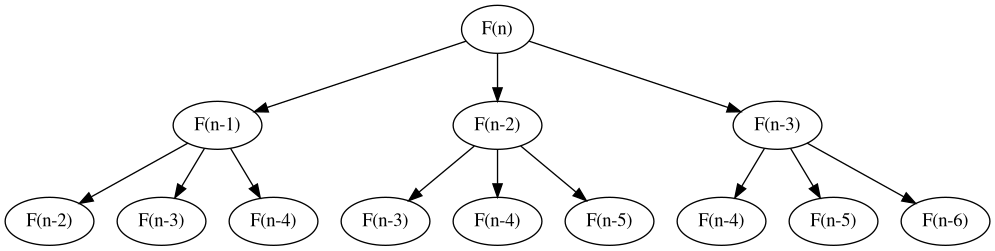
\includegraphics[width=0.8\textwidth]{fib_daq.png}
	\end{center}

	We can see that this approach is highly inefficent as subproblems are solved multiple times in the recursive tree. The time complexity can be defined recursively as T(n) = T(n-1) + T(n-2) + T(n-3), which leads to a complexity in the order of $\mathcal{O}(3^n)$.
	
\end{enumerate}


\end{document}
